% !TeX root = ../tfg.tex
% !TeX encoding = utf8

\chapter{Categorías}\label{ch:categorias}

\section{Introducción}
Este documento es una plantilla para la elaboración de un trabajo fin de Grado siguiendo los \href{https://grados.ugr.es/matematicas/pages/infoacademica/tfg/requisitosTFG}{requisitos} de la comisión de Grado en Matemáticas de la Universidad de Granada que, a fecha de junio de 2023, son las siguientes:

\begin{itemize}
  \item La  memoria  debe  realizarse  con  un  procesador  de  texto  científico,  preferiblemente (La)TeX.
  \item La portada  debe contener  el  logo  de  la UGR,  incluir  el  título del TFG, el nombre del estudiante y especificar el grado, la facultad y el curso actual.
  \item La contraportada contendrá además el nombre del tutor o tutores.
  \item La memoria debe necesariamente incluir:
    \begin{itemize}
      \item Declaración explícita firmada en la que se asume la originalidad del trabajo, entendida en el sentido de que no ha utilizado fuentes sin citarlas debidamente. Esta declaración se puede descargar en la web del Grado.
      \item un índice detallado de capítulos y secciones,
      \item un resumen amplio en inglés del trabajo realizado (se recomienda entre 800 y 1500 palabras),
      \item una introducción en la que se describan claramente los objetivos previstos inicialmente en la propuesta de TFG, indicando si han sido o no alcanzados, los antecedentes importantes para el desarrollo, los resultados obtenidos, en su caso y las principales fuentes consultadas,
      \item una bibliografía final que incluya todas las referencias utilizadas.
    \end{itemize}
  \item Se recomienda que la extensión de la memoria sea de unas 50 páginas, sin incluir posibles apéndices.
\end{itemize}

Para generar el pdf a partir de la plantilla basta compilar el fichero \texttt{tfg.tex}. Es conveniente leer los comentarios contenidos en dicho fichero pues ayudarán a entender mejor como funciona la plantilla. 

La estructura de la plantilla es la siguiente\footnote{Los nombres de las carpetas no se han acentuado para evitar problemas en sistemas con Windows}: 
\begin{itemize}
  \item Carpeta \textbf{preliminares}: contiene los siguientes archivos
    \begin{description}
      \item[\texttt{dedicatoria.tex}] Para la dedicatoria del trabajo (opcional)
      \item[\texttt{agradecimientos.tex}] Para los agradecimientos del trabajo (opcional)
      \item[\texttt{introduccion.tex}] Para la introducción (obligatorio)
      \item[\texttt{summary.tex}] Para el resumen en inglés (obligatorio)
      \item[\texttt{tablacontenidos.tex}] Genera de forma automática la tabla de contenidos, el índice de figuras y el índice de tablas. Si bien la tabla de contenidos es conveniente incluirla, el índice de figuras y tablas es opcional. Por defecto está desactivado. Para mostrar dichos índices hay que editar este fichero y quitar el comentario a \verb+\listoffigures+ o \verb+\listoftables+ según queramos uno de los índices o los dos. En este archivo también es posible habilitar la inclusión de un índice de listados de código (si estos han sido incluidos con el paquete \texttt{listings})
  \end{description}
  El resto de archivos de dicha carpeta no es necesario editarlos pues su contenido se generará automáticamente a partir de los metadatos que agreguemos en \texttt{tfg.tex}

  \item Carpeta \textbf{capitulos}: contiene los archivos de los capítulos del TFG. Añadir tantos archivos como sean necesarios. Este capítulo es \texttt{capitulo01.tex}.

  \item Carpeta \textbf{apendices}: Para los apéndices (opcional)
  \item Carpeta \textbf{img}: Para incluir los ficheros de imagen que se usarán en el documento.
    
  \item Fichero \texttt{library.bib}: Para incluir las referencias bibliográficas en formato \texttt{bibtex}. Es útil la herramienta \href{https://www.doi2bib.org/}{doi2bib} para generar de forma automática el código bibtex de una referencia a partir de su \textsc{doi}  así como la base de datos bibliográfica \href{https://mathscinet.ams.org}{MathSciNet}. Para que una referencia aparezca en el pdf no basta con incluirla en el fichero \texttt{library.bib}, es necesario además \emph{citarla} en el documento usando el comando \verb+\cite+. Si queremos mostrar todos las referencias incluidas en el fichero \texttt{library.bib} podemos usar \verb+\cite{*}+ aunque esta opción no es la más adecuada. Se aconseja que los elementos de la bibliografía estén citados al menos una vez en el documento (y de esa forma aparecerán de forma automática en la lista de referencias).

  \item Fichero \texttt{glosario.tex}: Para incluir un glosario en el trabajo (opcional). Si no queremos incluir un glosario deberemos borrar el comando \verb+\input{glosario.tex}+ del fichero \texttt{tfg.tex} y posteriormente borrar el fichero \texttt{glosario.tex}

   \item Fichero \texttt{tfg.tex}: El documento maestro del TFG que hay que compilar con \LaTeX\ para obtener el pdf. En dicho documento hay que cambiar la \emph{información del título del \textsc{tfg} y el autor así como los tutores}.
\end{itemize}

\section{Definición y propiedades}

\begin{definicion}\label{def_categoria}
    Una categoría $\mathscr{C}$ consiste en:
    \begin{enumerate}
        \item Una clase $|\mathscr{C}|$ cuyos elementos se llamarán ``objetos de la categoría'';
        \item Para cada par $A,B$ de objetos, un conjunto $\mathscr{C}(A,B)$, conocido como homset, cuyos elementos llamaremos ``morfismos'' ó ``flechas'' desde $A$ hasta $B$;
        \item Para cada $A,B,C \in |\mathscr{C}|$, se define una ley de composición:
            \begin{equation}
                \mathscr{C}(A,B) \times \mathscr{C}(B,C) \longrightarrow \mathscr{C}(A,C)
            \end{equation}
        la composición del par $(f,g)$ se notará como $g\circ f$, ó simplemente $gf$;
        \item Para cada objeto $A$, un morfismo $1_{A} \in \mathscr{C}(A,A)$ que llamaremos la identidad en $A$.
    \end{enumerate}
\end{definicion}

En una categoría encontramos los siguientes axiomas o propiedades:

\begin{enumerate}
    \item \textit{Asociatividad: } dados los morfismos $f \in \mathscr{C}(A,B)$, $g \in \mathscr{C}(B,C)$, $h \in \mathscr{C}(C,D)$, la siguiente igualdad se cumple:
        \begin{equation}
            h \circ (g \circ f) = (h \circ g) \circ f.
        \end{equation}
    Esto es, la ley de composición de morfismos es asociativa.    
    \item \textit{Identidad: } dados los morfismos $f \in \mathscr{C}(A,B)$, $g \in \mathscr{C}(B,C)$ la siguiente igualdad se cumple: 
        \begin{equation}
            1_{B} \circ f = f, \quad g \circ 1_{B} = g 
        \end{equation}
\end{enumerate}

\begin{figure}[htpb] % El entorno figure permite añadir el título
    \centering
    \begin{tikzcd}[row sep=2cm, column sep=2cm]
        A \arrow{r}{f} \arrow{d}[left]{h} 
        & B \arrow{d}{g}  \\
        C \arrow{r}{k} 
        & D
    \end{tikzcd}
    \caption{Diagrama conmutativo}
    \label{diag:diagrama-basico}
\end{figure}

Un morfismo $f \in \mathscr{C}(A,B)$ normalmente se representará mediante la notación con flecha $f: A \longrightarrow B$, donde $A$ se conoce como ``dominio'' y $B$ como ``codominio''.
En la situación del diagrama \ref{diag:diagrama-basico}, diremos que dicho diagrama es ``conmutativo'' si se da la igualdad $gf = kh$. El concepto de ``conmutatividad'' se mantiene para diagramas de dimensión aritraria. \\
El morfismo identidad $1_{A}$ de un objeto $A$ es el único morfismo cumpliendo el rol de identidad para la composición. Esto es, si $i_{A} \in \mathscr{C}(A,A)$ cumple dicha propiedad, entonces:

\begin{equation}
    1_{A} = 1_{A} \circ i_{A} = 1_{A}
\end{equation}

Una forma importante de construir categorías a partir de una categoría dada se recoge en la siguiente definición.

\begin{definicion}
    (Categoría opuesta): Toda categoría $\mathscr{A}$ tiene una categoría \textit{opuesta} $\mathscr{A}^{op}$ definida:
    \begin{enumerate}
        \item $|\mathscr{A}^{op}| = |\mathscr{A}|$,
        \item $\mathscr{A}^{op}(B,A) = \mathscr{A}(A,B) \, \, \, , \forall A,B \in \mathscr{A}^{op}$,
        \item En cuanto a la composición, si tenemos los morfismos $A \xlongrightarrow{f} B \xlongrightarrow{g} C $ en $\mathscr{A}^{op}$, entonces en $\mathscr{A}$ nos encontramos  $A \xlongleftarrow{f} B \xlongleftarrow{g} C $. En $\mathscr{A}^{op}$ encontramos la composición $g \circ f: A \longrightarrow C$ y en $\mathscr{A}$ tenemos $f \circ g: A \longleftarrow C$
    \end{enumerate}
    Por tanto, los morfismos $f: A \longrightarrow B$ en $\mathscr{A}$ se corresponden con los morfismos $f: B \longrightarrow A$ en $\mathscr{A}^{op}$.
\end{definicion}

Una propiedad importante en teoría de categorías es el \textit{principio de dualidad}, que relaciona las propiedades que se dan en una categoría $\mathscr{A}$ y su opuesta $\mathscr{A}^{op}$.

\section{Ejemplos}
Veamos algunos ejemplos:

\begin{ejemplo}
    \textbf{Set: } 
    \begin{itemize}
        \item \textbf{Objetos: } Conjuntos
        \item \textbf{Morfismos: } funciones entre conjuntos
    \end{itemize}
\end{ejemplo}

\begin{ejemplo}
    \textbf{Top: } 
    \begin{itemize}
        \item \textbf{Objetos: } Espacios topológicos
        \item \textbf{Morfismos: } funciones continuas
    \end{itemize}
\end{ejemplo}

\begin{ejemplo}
    \textbf{Grp: } 
    \begin{itemize}
        \item \textbf{Objetos: } Grupos
        \item \textbf{Morfismos: } homomorfismos de grupos
    \end{itemize}
\end{ejemplo}

\begin{ejemplo}
    Sea $I \in \mathscr{C}$ definimos la categoría de flechas sobre $I$, notada como $\mathscr{C}/I$, como sigue:
    \begin{itemize}
        \item \textbf{Objetos: } las flechas cuyo codominio es $I$
        \item \textbf{Morfismos: } los morfismos de un objeto $(f: A \longrightarrow I)$ a $(g: B \longrightarrow I)$ forman el conjunto de morfismos $h: A \longrightarrow B$ de $\mathscr{C}$ cumpliendo $g \circ h = f$ (ver diagrama \ref{diag:traingulo_hacia})
    \end{itemize}
\end{ejemplo}

\begin{figure}[htpb]
    \centering
    \begin{tikzcd}[row sep=1cm, column sep=1cm]
        A \arrow{dr}[below left]{f} \arrow{rr}{h} 
        & & B \arrow{ld}{g}  \\
        & I
    \end{tikzcd}
    \caption{Triángulo conmutativo}
    \label{diag:traingulo_hacia}
\end{figure}

\begin{ejemplo}
    En la misma línea que el anterior ejemplo, definimos la categoría de morfismos que parten del objeto $I$ de $\mathscr{C}$, notada como $I / \mathscr{C}$ como sigue: 
    \begin{itemize}
        \item \textbf{Objetos: } las flechas cuyo dominio es $I$
        \item \textbf{Morfismos: } los morfismos de un objeto $(f: I \longrightarrow A)$ a $(g: I \longrightarrow B)$ forman el conjunto de morfismos $h: A \longrightarrow B$ de $\mathscr{C}$ cumpliendo $h \circ f = g$ (ver diagrama \ref{diag:traingulo_desde})
    \end{itemize}
\end{ejemplo}

\begin{figure}[htpb]
    \centering
    \begin{tikzcd}[row sep=1cm, column sep=1cm]
        & I \arrow{dl}[above]{f} \arrow{dr}{g} & \\
        A \arrow{rr}[below]{h} & & B
    \end{tikzcd}
    \caption{Triángulo conmutativo}
    \label{diag:traingulo_desde}
\end{figure}

\begin{ejemplo}
    Definimos ahora la categoría de flechas de una categoría $\mathscr{C}$, notada como $\textbf{Ar}(\mathscr{C})$ de la siguiente forma:
    \begin{itemize}
        \item \textbf{Objetos: } todas las flechas de $\mathscr{C}$
        \item \textbf{Morfismos: } un morfismo de un objeto $(f: A \longrightarrow B)$ a $(g: C \longrightarrow D)$ es un par $(h: A \longrightarrow C, k: B \longrightarrow D)$ de morfismos de $\mathscr{C}$ cumpliendo $k \circ f = h \circ g$ (ver diagrama \ref{diag:diagrama-flechas})
    \end{itemize}
\end{ejemplo}

\begin{figure}[htpb] % El entorno figure permite añadir el título
    \centering
    \begin{tikzcd}[row sep=2cm, column sep=2cm]
        A \arrow{r}{f} \arrow{d}[left]{h} 
        & B \arrow{d}{k}  \\
        C \arrow{r}{g} 
        & D
    \end{tikzcd}
    \caption{Morfismo de flechas}
    \label{diag:diagrama-flechas}
\end{figure}

%--------------------FUNCTORES-------------------------

\section{Functores}
\subsection{Definición y propiedades}
Una vez definido el concepto de categoría y sus principales propiedades, veamos ahora el concepto que recoge las correspondencias entre categorías.

\begin{definicion}
    Un functor $F$ de una categoría $\mathscr{A}$ a una categoría $\mathscr{B}$ consiste en:

    \begin{enumerate}
        \item una función \begin{equation}|\mathscr{A}| \longrightarrow |\mathscr{B}| \end{equation} entre las clases de objetos de las categorías; la imagen de un objeto $A \in \mathscr{A}$ se nota $F(A)$ o simplemente $FA$.

        \item para cada $A, A' \in \mathscr{A}$, una función \begin{equation}\mathscr{A}(A,A') \longrightarrow \mathscr{B}(FA,FA') \end{equation}
        la imagen de un morfismo $f \in \mathscr{A}(A,A')$ se nota como $F(f)$ o simplemente $Ff$.
    \end{enumerate}
    \label{functor}
\end{definicion}

\begin{observacion} Las siguientes propiedades aseguran que los functores respeten la estructura subyacente de las categorías donde se definene.
  \begin{enumerate}
        \item para cada par de morfismos $f \in \mathscr{A}(A,A')$, $g \in          \mathscr{A}(A',A''): $ \begin{equation} F(g \circ f) = F(g) \circ F(f)   \end{equation}

        \item para cada $A \in \mathscr{A}$ \begin{equation}
            F(1_{A}) = 1_{FA}
        \end{equation}
    \end{enumerate}  
\end{observacion}

\begin{observacion}
    Dados dos functores $F: \mathscr{A} \longrightarrow {B}$ y $G: \mathscr{B} \longrightarrow {C}$ se puede definir una composición sobre objetos que produce un nuevo functor $G \circ F: \mathscr{A} \longrightarrow \mathscr{C}$. Esta composición cumple:

    \begin{enumerate}
        \item \textit{Asociatividad: } Dados los functores $F: \mathscr{A} \longrightarrow \mathscr{B}$, $G: \mathscr{B} \longrightarrow \mathscr{C}$ y $H: \mathscr{C} \longrightarrow \mathscr{D}$, se cumple: \begin{equation}
            H \circ (G \circ F) = (H \circ G) \circ F   
        \end{equation}
        \item \textit{Identidad: } Para cada categoría $\mathscr{A}$ existe un functor identidad $id_A: \mathscr{A} \longrightarrow \mathscr{A}$ (cuya definición es evidente) de forma que si $F: \mathscr{A} \longrightarrow \mathscr{B}$ es otro functor, se cumple \begin{equation}
            F \circ id_{\mathscr{A}} = id_{\mathscr{B}} \circ F 
        \end{equation} 
    \end{enumerate}
\end{observacion}

A primera vista puede parecer que las categorías como objetos y los functores como morfismos entre ellas cumplen todos los axiomas de las categorías.  Sin embargo, recordemos que los morfismos entre objetos deben formar un conjunto. Por tanto, para que las categorías y sus functores puedan formar una categoría, se debe cumplir que el objeto que contenga a todos los functores entre dos categorías sea un conjunto. Esto no sucede siempre, pero el motivo queda fuera del ámbito de este trabajo.

\subsection{Ejemplos}
Veamos algunos ejemplos de functores:

\begin{ejemplo}
    El ``forgetful functor'' (o functor olvidadizo, haciendo una traducción literal) $U: \textbf{Ab} \longrightarrow \textbf{Set} $ de la categoría de grupos abelianos a la categoría de conjuntos, lleva un grupo $(G,+)$ en su conjunto asociado $G$ y un homomorfismo de grupos $f$ en una función entre los conjuntos asociados $f$. Debe su nombre a que dicho functor ``olvida'' la estructura subyacente de grupo.
    \label{ej:forgetful}
\end{ejemplo}

\begin{ejemplo}
     La categoría $\textbf{Top}_{*}$ de espacios topológicos con punto base tiene como objetos duplas $(X,x_{0})$ donde:
    \begin{itemize}
        \item $X$ es un espacio topológico.
        \item $x_{0} \in X$ es un punto base de dicho espacio 
    \end{itemize}
    Los morfismos de $\textbf{Top}_{*}$ son funciones $f: (X,x_{0}) \longrightarrow (Y,y_{0})$ cumpliendo:
    \begin{itemize}
        \item $f$ es una función continua entre $X$ e $Y$.
        \item $f(x_{0}) = y_{0}$ 
    \end{itemize}
    El grupo fundamental se puede definir como un functor $\pi_{1}: \textbf{Top}_{*} \longrightarrow \textbf{Grp} $ que asigna a cada espacio con punto base $(X,x_{0})$ su grupo fundamental $\pi_{1}(X,x_{0})$, y a cada función continua entre espacios base $f: (X,x_{0}) \longrightarrow (Y,y_{0})$ el homomorfismo de grupos asociado $f_{*}: \pi_{1}(X,x_{0}) \longrightarrow \pi_{1}(Y,y_{0})$
\end{ejemplo}

\begin{ejemplo}
    El functor $\mathcal{P}: \textbf{Set} \longrightarrow \textbf{Set}$ lleva un conjunto $X$ en su conjunto potencia $\mathcal{P}(X)$ y una función $f: X \longrightarrow Y$ a una función $\mathcal{P}(f): \mathcal{P}(X) \longrightarrow \mathcal{P}(Y)$ que asigna a cada subconjunto $A \subseteq X$ el subconjunto $f(A) \subseteq Y$, esto es $f(A) = \{f(a) : a \in A\} \subseteq Y$.
    \label{ejemplo:potencia}
\end{ejemplo}

\begin{ejemplo}
    Otro functor importante en teoría de categorías es el functor representable. Dada una categoría $\mathscr{C}$ y un objeto $C \in \mathscr{C}$, se define el functor \begin{equation}
        \mathscr{C}(C,-): \mathscr{C} \longrightarrow Set
    \end{equation} que asocia a cada objeto $A \in \mathscr{C}$ el objeto $\mathscr{C}(C,A)$ de la clase \textbf{Set}. \\
    Si $f: A \longrightarrow B$ es un morfismo en $\mathscr{C}$, la imagen por el functor representable será una función entre conjuntos de la siguiente forma: \begin{equation}
        \mathscr{C}(C,-)(f): \mathscr{C}(C,A) \longrightarrow \mathscr{C}(C,B)
    \end{equation} de forma que para cada $g \in \mathscr{C}(C,A)$ obtenemos un morfismo $f \circ g: C \longrightarrow B$, esto es, $f \circ g \in \mathscr{C}(C,B).$
    Este functor se conoce como representable ya que es ``representado'' por el objeto $C$, en el sentido de que si conocemos el objeto $C$ y como se relaciona con el resto de morfismos de su categoría, conocemos su functor representable. 
    \label{ej:func_repre}
\end{ejemplo}

\subsection{Functores contravariantes}
Definimos ahora un concepto central en este trabajo.

\begin{definicion}
    (Functor contravariante) Un functor contravariante $F$ de una categoría $\mathscr{A}$ a una categoría $\mathscr{B}$ consiste en:

    \begin{enumerate}
        \item una función \begin{equation}|\mathscr{A}| \longrightarrow |\mathscr{B}| \end{equation} entre las clases de objetos de las categorías; la imagen de un objeto $A \in \mathscr{A}$ se nota $F(A)$ o simplemente $FA$.

        \item para cada $A, A' \in \mathscr{A}$, una función \begin{equation}\mathscr{A}(A,A') \longrightarrow \mathscr{B}(FA',FA) \end{equation}
        la imagen de un morfismo $f \in \mathscr{A}(A,A')$ se nota como $F(f)$ o simplemente $Ff$.
    \end{enumerate}
\end{definicion}

\begin{observacion} Las siguientes propiedades aseguran que los functores respeten la estructura subyacente de las categorías donde se definene.
  \begin{enumerate}
        \item para cada par de morfismos $f \in \mathscr{A}(A,A')$, $g \in          \mathscr{A}(A',A''): $ \begin{equation} F(g \circ f) = F(f) \circ F(g)   \end{equation}

        \item para cada $A \in \mathscr{A}$ \begin{equation}
            F(1_{A}) = 1_{FA}
        \end{equation}
    \end{enumerate}  
\end{observacion}

Para evitar confusiones, enfatizaremos que estamos trabajando con un functor como el definido en \ref{functor} llamándolo functor \emph{covariante}. Un functor contravariante $F: \mathscr{A} \longrightarrow \mathscr{B}$ es un functor covariante entre las categorías $\mathscr{A}^{op}$ y $\mathscr{B}$.

\subsubsection{Ejemplos}

Veamos algunos ejemplos de functores contravariantes.

\begin{ejemplo}
    Análogo al functor representable definido en \ref{ej:func_repre}, encontramos el siguiente functor contravariante:

    Dada una categoría $\mathscr{C}$ y un objeto $C \in \mathscr{C}$, se define el functor \begin{equation}
        \mathscr{C}(-,C): \mathscr{C} \longrightarrow Set
    \end{equation} que asocia a cada objeto $A \in \mathscr{C}$, el objeto $\mathscr{C}(A,C)$ de la clase \textbf{Set}. \\
    Si $f: A \longrightarrow B$ es un morfismo en $\mathscr{C}$, la imagen por el functor representable será una función entre conjuntos de la siguiente forma: \begin{equation}
        \mathscr{C}(-,C)(f): \mathscr{C}(B,C) \longrightarrow \mathscr{C}(A,C)
    \end{equation} de forma que para cada $g \in \mathscr{C}(B,C)$ obtenemos un morfismo $g \circ f: A \longrightarrow B$, esto es, $g \circ f \in \mathscr{C}(A,C).$    
\end{ejemplo}

\section{Transformaciones naturales}
\subsection{Definición y propiedades}
En matemáticas siempre se suele comenzar estudiando los objetos y posteriormente las transformaciones entre ellos. En el apartado anterior hemos visto como los functores ``transforman'' una categoría en otra, respetando la estructura de la categoría. Nos proponemos ahora tratar los functores como objetos y definir transformaciones entre ellos que respeten las estructuras categóricas subyacentes. 

\begin{figure}[htpb]
    \centering
    \begin{tikzcd}[row sep=2cm, column sep=2cm]
        FA \arrow{r}{\alpha_{A}} \arrow{d}[left]{F(f)} 
        & GA \arrow{d}{G(f)}  \\
        FA' \arrow{r}{\alpha_{A'}} 
        & GA'
    \end{tikzcd}
    \caption{Diagrama conmutativo}
    \label{diag:trans_natural}
\end{figure}

\begin{definicion}
    Sean dos functores $F,G: \mathscr{A} \longrightarrow \mathscr{B}$ de una categoría $\mathscr{A}$ a una categoría $\mathscr{B}$. Una transformación natural $\alpha: F \Rightarrow G$ de $F$ a $G$ es una clase de morfismos $(\alpha_A:FA \longrightarrow GA)_{A\in \mathscr{A}}$ cumpliendo que para cada morfismo $f: A \longrightarrow A'$ se cumple \begin{equation}
        G(f) \circ \alpha_{A} = \alpha_{A'} \circ F(f)
    \end{equation}
    (ver diagrama \ref{diag:trans_natural})
    \label{t_natural}
\end{definicion}

\begin{figure}[htpb]
    \centering
    \begin{tikzcd}[row sep=huge]
        \mathscr{A}
        \arrow[bend left=65]{r}{F}
        \arrow[r, "G"{inner sep=0,fill=white,anchor=center,name=G}]
        \arrow[r, bend right=65, "H"{name=H, swap}]
        \arrow[from=F.south-|G,to=G,Rightarrow,shorten=2pt,"\alpha"] 
        \arrow[from=G,to=H.north-|G,Rightarrow,shorten=2pt,"\beta"] &
        \mathscr{B}.
    \end{tikzcd}
\end{figure}

\begin{definicion}
        Dados $F,G,H$ functores de $\mathscr{A}$ a $\mathscr{B}$ y $\alpha: F \Rightarrow G$, $\beta: G \Rightarrow H$ se define la composición (vertical) de transformaciones naturales, $(\beta \circ \alpha)_{A}: F \Rightarrow H$, mediante la fórmula \begin{equation}
        (\beta \circ \alpha)_{A} = \beta_{A} \circ \alpha_{A}
    \end{equation}
    
    Esta composición cumple:
    
    \begin{enumerate}
        \item \textit{Asociatividad: } Dados $F,G,H, K$ functores de $\mathscr{A}$ a $\mathscr{B}$ y $\alpha: F \Rightarrow G$, $\beta: G \Rightarrow H$, $\delta: H \Rightarrow K$ transformaciones naturales, se cumple: \begin{equation}
            \delta \circ (\beta \circ \alpha) = (\delta \circ \beta) \circ \alpha
        \end{equation} 
        \item \textit{Identidad: }  Para cada functor $F: \mathscr{A} \longrightarrow \mathscr{B}$ existe una transformación natural $id_{F}: F \Rightarrow F$ que cumple el papel de identidad para la composición, de forma que si $G: \mathscr{A} \longrightarrow \mathscr{B}$ es otro functor y $\alpha: F \Rightarrow G$ es una transformación natural: \begin{equation}
            \alpha \circ id_{F} = id_{G} \circ \alpha
        \end{equation}
    \end{enumerate}
\end{definicion}

De forma análoga a como hemos discutido antes en el caso de las categorías y los functores, vemos que los functores entre $\mathscr{A}$ y $\mathscr{B}$ como objetos y las transformaciones naturales como morfismos entre ellos cumplen los axiomas que caracterizan a una categoría. Sin embargo, al igual que en el caso de los functores, no tenemos garantizado que el objeto que contiene todas las transformaciones naturales entre dos functores sea un conjunto. Con algunas condiciones extra, esta condición se cumple y los functores junto con las transformaciones naturales forman una categoría.

Una forma intuitiva de entender las transformaciones naturales es de la siguiente forma: cuando aplicamos un functor en una categoría, asociamos a cada objeto un objeto, y a cada morfismo un morfismo. Sin embargo, en una transformación natural asignamos a cada objeto $A \in \mathscr{A}$ un morfismo $(\alpha_{A})$ y a cada morfismo $f: A \longrightarrow A'$ un diagrama cuadrado como el visto en el diagrama \ref{diag:trans_natural}. Por tanto, si vemos las categorías como objetos $0$-$dimensionales$ y los functores como objetos $1$-$dimensionales$, las transformaciones naturales serían objetos $2$-$dimensionales$. 

\subsection{Ejemplos}
Veamos algunos ejemplos de transformaciones naturales.

\begin{ejemplo}
    Sean el functor potencia en la categoría \textbf{Set}, definido en \ref{ejemplo:potencia}, y el functor identidad $id: \textbf{Set} \longrightarrow \textbf{Set}$. La transformación natural $\alpha: id \Rightarrow \mathcal{P}$ definida como $\alpha_{E}: E \longrightarrow \mathcal{P}(E)$ lleva cada elemento $x \in E$ al singleton ${x} \in \mathcal{P}(E)$.
\end{ejemplo}

\begin{ejemplo}
    Sea una categoría $\mathscr{A}$ y un morfismo $f:A \longrightarrow B$ de $\mathscr{A}$. De los siguientes functores representables obtenemos una transformación natural $\mathscr{A}(f,-) : \mathscr{A}(B,-) \Rightarrow \mathscr{A}(A,-)$  que asocia a cada objeto $C \in \mathscr{A}$ una función entre conjuntos $\mathscr{A}(f,-)_{C}: \mathscr{A}(B,C) \longrightarrow \mathscr{A}(A,C)$ definida como \begin{equation}
        \mathscr{A}(f,-)_{C}(g) = g \circ f
    \end{equation}
\end{ejemplo}

\subsection{Transformaciones naturales de functores contravariantes}
La definición hecha en \ref{t_natural} corresponde a transformaciones naturales de functores covariantes. De forma análoga se definen las transformaciones naturales entre functores contravariantes. 

\begin{figure}[htpb]
    \centering
    \begin{tikzcd}[row sep=2cm, column sep=2cm]
        FA \arrow{r}{\alpha_{A}} 
        &  GA \\
        FA' \arrow{r}{\alpha_{A'}} \arrow{u}[left]{F(f)}
        & GA' \arrow{u}{G(f)} 
    \end{tikzcd}
    \caption{Diagrama conmutativo}
    \label{diag:trans_natural_contra}
\end{figure}

\begin{definicion}
    Sean dos functores contravariantes $F,G: \mathscr{A} \longrightarrow \mathscr{B}$ de una categoría $\mathscr{A}$ a una categoría $\mathscr{B}$. Una transformación natural $\alpha: F \Rightarrow G$ de $F$ a $G$ es una clase de morfismos $(\alpha_A:FA \longrightarrow GA)_{A\in \mathscr{A}}$ cumpliendo que para cada morfismo $f: A \longrightarrow A'$ se cumple \begin{equation}
        G(f) \circ \alpha_{A'} = \alpha_{A} \circ F(f)
    \end{equation}
    (ver diagrama \ref{diag:trans_natural_contra})
    \label{t_natural}    
\end{definicion}

\section{Subcategorías}

\begin{definicion}
    Sea el functor $F: \mathscr{A} \longrightarrow \mathscr{B}$ y para cada par de objetos $A,A' \in \mathscr{A}$ la función \begin{equation}
        \mathscr{A}(A,A') \longrightarrow \mathscr{B}(FA,FA'), \, \, \, f \mapsto Ff
    \end{equation}
    \begin{enumerate}
        \item Decimos que el functor F es \textit{faithful} si la función definida arriba es inyectiva para cada $A,A'$.
        \item Decimos que el functor F es \textit{full} si la función definida arriba es sobreyectiva para cada $A,A'$.
        \item Decimos que el functor F es \textit{full} y \textit{faithful} si la función definida arriba es biyectiva para cada $A,A'$.
        \item El functor F es un isomorfismo de categorías cuando es \textit{full} y \textit{faithful} e induce una biyección $|\mathscr{A}| \longrightarrow |\mathscr{B}|$ entre las clases de objetos.
    \end{enumerate}
\end{definicion}

Damos ahora el concepto de subcategoría:

\begin{definicion}
    Una subcategoría $\mathscr{B}$ de una categoría $\mathscr{A}$ consiste en:
    \begin{enumerate}
        \item Una subclase $|\mathscr{B}| \subseteq |\mathscr{A}|$ de la clase de objetos,
        \item Para cada par de objetos $A,A' \in \mathscr{B}$, un subconjunto $\mathscr{B}(A,A') \subseteq \mathscr{A}(A,A')$ de forma que 
        \begin{enumerate}
            \item $f \in \mathscr{B}(A,A')$ y $g \in \mathscr{B}(A',A'') \implies g \circ f \in \mathscr{B}(A,A''),$ 
            \item $\forall A \in \mathscr{B}, 1_{A} \in \mathscr{B}(A,A).$
        \end{enumerate}

    \end{enumerate}
    De forma evidente, una subcategoría es una categoría. Además, una subcategoría $\mathscr{B}$ de $\mathscr{A}$ induce un functor inclusion $\mathscr{B} \longrightarrow \mathscr{A}$ que es \textit{faithful}.
\end{definicion}

Veamos un ejemplo interesante:
\begin{ejemplo}
    Recordemos el \textit{forgetful functor} definido en \ref{ej:forgetful} que asignaba a cada grupo $G \in \textbf{Grp}$ su estructura subyacente de conjunto en la categoría $\textbf{Set}$. Es evidente que se cumple $|Grp| \subseteq |Set|$. Además, para cada dos grupos $G, H \in \textbf{Grp}$, el conjunto de homomorfismos de grupos entre ellos, $\textbf{Grp}(G,H)$ está contenido en el conjunto $\textbf{Set}(G,H)$ de funciones entre los conjuntos subyacentes. Por tanto \textbf{Grp} es una subcategoría de $\textbf{Set}$, y el \textit{forgetful functor} define la inclusión entre ambas categorías (esto es, el \textit{forgetful functor} es \textit{faithful}).
\end{ejemplo}

\section{Límites y colímites}

Vamos a empezar viendo algunos ejemplos comunes del concepto de límite, con el objetivo de tener una visión más general una vez enunciemos la definición.

\subsection{Producto}

\begin{definicion}
    (Producto): Sea $\mathscr{C}$ una categoría y $A,B \in \mathscr{C}$ dos objetos. Un producto de $A,B$ consiste en un objeto $P$ y morfismos:

    \begin{center}
        \begin{tikzcd}[row sep=1cm, column sep=1cm]
            &  P \arrow{ld}[swap]{p_{A}} \arrow{rd}{p_{B}} & \\
            A & & B
        \end{tikzcd}
    \end{center}
    de forma que para cada objeto $Q$ y morfismos


    \begin{figure}[htpb]
        \centering
        \begin{tikzcd}[row sep=1cm, column sep=1cm]
            &  Q \arrow{ld}[swap]{q_{A}} \arrow{rd}{q_{B}} & \\
            A & & B
        \end{tikzcd}
        \label{diag:producto}
    \end{figure}
        
    en $\mathscr{C}$, existe un \textbf{único} morfismo $\bar{f}: Q \longrightarrow P$ tal que 

    \begin{figure}[htpb]
        \centering
        \begin{tikzcd}[row sep=1cm, column sep=1cm]
            & Q \arrow[dashed]{d}[description]{\exists! \ \bar{f}} \arrow{ld}[swap]{q_A} \arrow{rd}{q_B} & \\
            A & P \arrow{l}[swap]{p_{A}} \arrow{r}{p_{B}} & B
        \end{tikzcd}
        \caption{Propiedad universal del producto}
        \label{diag:universal-producto}
    \end{figure}
    conmuta. 
    
    Esto se conoce como propiedad universal del producto. El producto es el objeto (y morfismos) ``más general'' que cumple las condiciones de las proyecciones $p_{A}$ y $p_{B}$.
    Lo notaremos como $(P, p_{A}, p_{B})$
    
\end{definicion}

\begin{proposicion}
    En una categoría \mathscr{C} el producto de dos objetos $A,B \in \mathscr{C}$ (si existe) es único salvo isomorfismo.
    $(P, \pi_{1}, \pi_{2})$
\end{proposicion}
\textit{Demostración.} Notar que el producto no siempre existe.  Por ejemplo, consideremos la categoría discreta 
$\mathscr{A}$ formada únicamente por los objetos $A$ y $B$. En esta categoría no puede existir el producto de $A$ y $B$.

Veamos ahora la unicidad salvo isomorfismo. Consideremos en la categoría \mathscr{C} dos productos $(P, p_A, p_B)$ y $(Q, q_A, q_B)$ de los
objetos $A,B \in \mathscr{C}$. Como $(P, p_A, p_B)$ es un prodcuto, existe un único morfismo $\bar{f}: Q \longrightarrow P $ cumpliendo que 
$q_A = p_A \circ \bar{f}$ y  $q_B = p_B \circ \bar{f}$. De forma análoga, como $(Q, q_A, q_B)$ es un producto, existe un único morfismo 
$\bar{g}: P \longrightarrow Q $ cumpliendo $p_A = q_A \circ \bar{g}$ y  $p_B = q_B \circ \bar{g}$.


Veamos algunos ejemplos de productos en diferentes categorías:

\begin{ejemplo}
    En la categoría \textbf{Set}, el producto de dos conjuntos $X,Y$ es el producto cartesiano usual $X \times Y$, equipado con las proyecciones usuales $\pi_{1}$ y $\pi_{2}$. Sea un conjunto $A$ y morfismos $f_1$ y $f_2$ como en \ref{diag:producto}. Definimos $\bar{f}: A \longrightarrow X \times Y$ como $\bar{f}(a) = (f_1(a),f_2(a))$. Se cumple de manera evidente que $\pi_i \circ \bar{f} = f_i$ con $i=1,2$; luego el diagrama \ref{diag:universal-producto} conmuta. Hay que probar que $\bar{f}$ es la única función entre $A$ y $X \times Y$ que cumple esta propiedad. Supongamos $\hat{f}: A \longrightarrow X \times Y$ cumpliendo $\pi_i \circ \hat{f} = f_i$ con $i=1,2$. Tomemos $a \in A$ y sin pérdida de generalidad escribimos $\hat{f}(a) = (x,y)$. Como $\hat{f}$ hace conmutar a \ref{diag:universal-producto}, se cumple que $f_1(a) = p_1(\hat{f}(a)) = p_1((x,y)) = x$ , $f_2(a) = p_2(\hat{f}(a)) = p_2((x,y)) = y$. Luego $\hat{f}(a) = (x,y) = (f_1(a),f_2(a)) = \bar{f}(a)$, obteniendo la unicidad buscada.
\end{ejemplo}

\begin{ejemplo}
    En la categoría \textbf{Grp} encontramos un producto en el \textit{producto directo de grupos}. Dados dos grupos $G$ y $H$, se define su producto directo $G \times H$ como: 
    \begin{enumerate}
        \item El conjunto subyacente es el producto cartesiano $G\times H$, esto es, $(g,h) \in G \times H$ con $g \in G$ y $h \in H$.
        \item La operación en $G \times H$ se define como \begin{equation}
            (g_1,h_1) \cdot (g_2,h_2) = (g_1*g_2, \ h_1\circ h_2)
        \end{equation}
    \end{enumerate}
\end{ejemplo}

Podemos generalizar el concepto de producto en una categoría $\mathscr{A}$ de la siguiente forma.

\begin{definicion}
    Sea $\mathscr{A}$ una categoría e $I$ un conjunto y una familia de objetos $(X_i)_{i\in I}$. El producto de $(X_i)_{i\in I}$ consiste en un objeto $P$ y una familia de morfismos \begin{equation}
        (P \xlongrightarrow{\pi_i} X_i)_{i \in I}
    \end{equation}
    de forma que para cada objeto $A$ y morfismos \begin{equation}
        (A \xlongrightarrow{f_i} X_i)_{i \in I}
    \end{equation}
    existe un único morfismo $\bar{f}: A \longrightarrow P$ cumpliendo $f_i = \pi_i \circ \bar{f}$ para $i=1,2$.
\end{definicion}

Veamos otro ejemplo de límite que nos será útil más adelante. 

\begin{definicion}
    (Equalizer): Sea $\mathscr{A}$ una categoría y \begin{tikzcd}
        X \arrow[r, shift left]{s} \arrow[r, shift right]{t}
        & Y
    \end{tikzcd} objetos y morfismos en $\mathscr{A}$. Se define el equalizer de $s$ y $t$ como un objeto $E$ y un morfismo $E \xlongrightarrow{i} X$ de forma que \begin{tikzcd}
        E \arrow[r]
        & X \arrow[r, shift left]
        \arrow[r, shift right]
        & Y
    \end{tikzcd}  cumple $s \circ i = t \circ i$ y para cualquier otro objeto $A$ y morfismo $A \xlongrightarrow{j} X$ cumpliendo la propiedad anterior, se tiene un único morfismo $\hat{f}: A \longrightarrow E$ de forma que

    \begin{center}
        \begin{tikzcd}[row sep=1cm, column sep=1cm]
            A \arrow{rd}{j} \arrow[dotted]{d}[swap]{\hat{f}}\\
            E \arrow{r}[swap]{i} & X
        \end{tikzcd}
    \end{center}
    conmuta.
\end{definicion}

\begin{ejemplo}
    En la categoría \textbf{Set}, dados los conjuntos y funciones entre ellos \begin{tikzcd}
        X \arrow[r, shift left]{s} \arrow[r, shift right]{t}
        & Y
    \end{tikzcd}, definimos el equalizer como el conjunto \begin{equation}
        E = \{x \in X \ | \ s(x) = t(x)\}
    \end{equation} y la inclusión $i: E \longrightarrow X$. 
\end{ejemplo}

\begin{ejemplo}
    En la categoría \textbf{Grp} consideremos un par de grupos $G$ y $H$ junto con homomorfismos \begin{tikzcd}
        G \arrow[r, shift left]{s} \arrow[r, shift right]{t}
        & H
    \end{tikzcd} donde $\epsilon: G \longrightarrow H$ es el homomorfismo trivial y $\theta: G \longrightarrow H$ es un homomorfismo cualquiera. El núcleo de $\theta$ será el equalizer del anterior diagrama, esto es, un objeto $ker \theta$ junto con un homomorfismo \begin{tikzcd}
         ker \ \theta \arrow[hook]{r}{i} & G
    \end{tikzcd} cumpliendo $\theta \circ i = \epsilon \circ i \implies \theta(g) = 0 \ \forall g \in ker \ \theta $.
\end{ejemplo}

Hemos visto dos construcciones diferentes: productos y equalizers. La filosofía detrás de estas construcciones es la misma: se parte de unos objetos con (posiblemente) morfismos entre sí. Se pretende construir un objeto junto con morfismos a los objetos originales de forma que se cumpla una propiedad universal.  

En el caso de los productos, nuestro punto de partida son dos objetos 

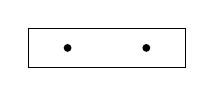
\begin{tikzpicture}
    \node[draw, rectangle, minimum width=2cm, minimum height=0.5cm] (boxT) {};
    \node[fill=black, circle, inner sep=1pt] at (-0.5, 0) {}; % Punto izquierdo
    \node[fill=black, circle, inner sep=1pt] at (0.5, 0) {}; % Punto derecho
\end{tikzpicture}      

\begin{definicion}
    
\end{definicion}

\section{Categorías abelianas}

\subsection{Conceptos previos}

\subsection{Definicion y propiedades}

\section{Adjunciones}

\section{Texto básico}

En esta sección presentaremos diferentes ejemplos de los elementos de texto básico. Conviene consultar el contenido de \texttt{capitulos/capitulo01.tex} para ver cómo se han incluido.

\subsection{Listas}
En \LaTeX\ tenemos disponibles los siguientes tipos de listas:

Listas enumeradas:
\begin{enumerate}
  \item item 1
  \item item 2
  \item item 3
\end{enumerate}

Listas no enumeradas
\begin{itemize}
  \item item 1
  \item item 2
  \item item 3
  \end{itemize}

Listas descriptivas
\begin{description}
  \item[termino1] descripción 1
  \item[termino2] descripción 2
\end{description}
  
\subsection{Tablas y figuras}

En la \autoref{tb:ejemplo-tabla} o la \autoref{fig:logo-ugr} podemos ver\ldots

\begin{table}[htpb]
  \centering
  \begin{tabular}{ccc} \toprule
    \multicolumn{2}{c}{Agrupados} \\ \cmidrule(r){1-2}
    cabecera & cabecera & cabecera          \\ \midrule
    elemento & elemento & elemento          \\ 
    elemento & elemento & elemento          \\ 
    elemento & elemento & elemento          \\ \bottomrule
  \end{tabular}
  \caption{Ejemplo de tabla}
  \label{tb:ejemplo-tabla}
\end{table}

\begin{figure}[htpb]
  \centering
  \includegraphics[width=0.5\textwidth]{logo-ugr}
  \caption{Logotipo de la Universidad de Granada}
  \label{fig:logo-ugr}
\end{figure}

\section{Formulas matematicas}\label{sec:functores}

La plantilla tiene definidos varios entornos matemáticos cuyo nombre es el mismo omitiendo los acentos. Así, para incluir una \emph{proposición} usaríamos:

\begin{verbatim}
\begin{proposicion}
texto de la proposición
\end{proposicion} 
\end{verbatim}

Ver el código fuente del archivo \texttt{documentacion.tex} en la carpeta \texttt{capitulos} para el resto de ejemplos.

\begin{teorema}\label{thm:teorema}
Esto es un ejemplo de teorema.
\end{teorema}

\begin{proposicion}
Ejemplo de proposición
\end{proposicion}

\begin{lema}
Ejemplo de lema
\end{lema}

\begin{corolario}
Ejemplo de corolario
\end{corolario}

\begin{definicion}
Ejemplo de definición
\end{definicion}

\begin{observacion}
Ejemplo de observación
\end{observacion}

Adicionalmente está definido el entorno \texttt{teorema*} que permite incluir un teorema sin numeración:

\begin{teorema*}[Fórmula de Gauß-Bonnet]
  Sea $S$ una superficie compacta y $K$ su curvatura de Gauß. Entonces
\begin{equation}
  \int_S K = 2\pi\chi(S)
\end{equation}
donde $\chi(S)$ es la característica de Euler de $S$.
\end{teorema*}

Las fórmulas matemáticas se escriben entre símbolos de dólar \$ si van en línea con el texto o bien usando el entorno%
\footnote{
  También es posible delimitar una ecuación mediante los comandos \texttt{$\backslash$[} y \texttt{$\backslash$]} pero éstas nunca llevarán numeración aunque añadamos una etiqueta y las referenciemos (ver \autoref{sec:referencias}).
} 
\texttt{equation} cuando queremos que se impriman centradas en una línea propia, como el siguiente ejemplo
\begin{equation}\label{eq:identidad-pitagorica}
  \cos^2 x + \sin^2 x = 1.
\end{equation}


Gracias al paquete \texttt{mathtools}, las ecuaciones escritas dentro del entorno \texttt{equation} llevarán numeración de forma automática si son referenciadas  en cualquier parte del documento (por ejemplo la identidad Pitagórica~\eqref{eq:identidad-pitagorica}, ver el código de los dos anteriores ejemplos y la \autoref{sec:referencias} para más información sobre referencias cruzadas en el documento).

\section{Código}

Podemos incluir un archivo externo de código mediante el comando \texttt{lstinputlisting} especificando su nombre completo (incluyendo la extensión) y usando la opción \texttt{inputpath} para indicar la ruta hacia el fichero (siempre referida a la carpeta principal de la plantilla) así como la opción \texttt{language} para indicar el lenguaje de programación en que está escrito (esto permitirá a \LaTeX\ colorear adecuadamente el código). Además, si lo consideramos necesario, podemos indicar las líneas que queremos mostrar (ver el código fuente del \autoref{code:prime}). Consultar todas las opciones posibles en la \href{https://osl.ugr.es/CTAN/macros/latex/contrib/listings/listings.pdf}{documentación del paquete \texttt{listings}}.

\lstinputlisting[inputpath=code, language=R, linerange={11-17}, firstnumber={11}, caption={Extracto código (líneas de 11 a 17) del fichero \texttt{primeR.r}}, label={code:prime}]{primeR.r}

Alternativamente, podemos incluir el código en un entorno \texttt{lstlisting} como el \autoref{code:perceptron}

\begin{lstlisting}[caption={Implementación de un perceptrón}, label={code:perceptron}, language={python}]
def dot(v, w):
    """Producto escalar de v y w, |$\color{comment}v_0 \cdot   w_0 + \cdots + v_n \cdot w_n$|"""
    return sum(v_i * w_i for v_i, w_i in zip(v, w))

def funcion_activacion(x):
    """1 si la entrada es mayor o igual que 1, 0 en otro caso."""
    return 1 if x >= 0 else 0

def perceptron(entrada, pesos):
    """1 si el perceptron se activa, 0 en otro caso"""
    return funcion_activacion(dot(entrada, pesos))
\end{lstlisting}

La opción \texttt{float} al incluir un listado de código permitará a dicho bloque ``flotar'' como si fuese un entorno \texttt{figure} y de esta manera evitaremos que se corte al final de una página.


\section{Referencias a elementos del texto}\label{sec:referencias}

Para las referencias a los elementos del texto (secciones, capítulos, teoremas,\ldots) se procede de la siguiente manera:
\begin{itemize}
  \item Se \emph{marca} el elemento (justo después del mismo si se trata de un capítulo o sección o en el interior del \emph{entorno} en otro caso), mediante el comando \verb+\label{+\emph{etiqueta}\verb+}+, donde \emph{etiqueta} debe ser un identificador único.
  \item Para crear una referencia al elemento en cualquier otra parte del texto se usa el comando \verb+\ref{+\emph{etiqueta}\verb+}+ (únicamente imprime la numeración asociada a dicho elemento, por ejemplo \ref{ch:primer-capitulo} o \ref{thm:teorema}) o bien \verb+\autoref{+\emph{etiqueta}\verb+}+ (imprime la numeración del elemento así como un texto previo indicando su tipo, por ejemplo \autoref{ch:primer-capitulo} o \autoref{thm:teorema})
\end{itemize}





\section{Bibliografía e índice}

Esto es un ejemplo de texto en un capítulo. Incluye varias citas tanto a libros~\cite{Aigner2018}, artículos de investigación~\cite{Euler1985}, recursos online~\cite{EulerWiki} (páginas web), tesis~\cite{CitekeyPhdthesis}, trabajo fin de máster~\cite{CitekeyMastersthesis}, trabajo fin de grado~\cite{CiteKeyBachelorsthesis} así como artículos sin publicar (preprints) \cite{castroinfantes2022conjugate} (en estos últimos usar el campo \texttt{note} para añadir la información relevante). 

Ver el fichero \texttt{library.bib} para las distintas plantillas. Cada nueva referencia debe añadirse en dicho fichero siguiendo el estilo del código \texttt{bibtex} según el tipo de referencia (página web, tesis, trabajo fin de grado o máster, artículo de investigación, libro,\ldots). Alternativamente se puede usar la web \href{https://zbib.org}{https://zbib.org} para generar automáticamente el código \texttt{bibtex}.


\endinput
